	\section{Цель работы}
		Изучить возможности и особенности инструментальных средств для создания гипертекста (ГТ) и гипертекстовых электронных справочных систем, а также получить навыки работы с ними и разработать электронную справочную систему для собственного программного приложения. 
	\section{Порядок выполенения работы}
	
		\subsection{Обзор современных средств создания гипертекстовых справочников}
		
		\textbf{HelpNDoc} Интерфейс и справка - на англ. языке.
		Назначение HelpNDoc - создание справок, различной документации и eBooks. HelpNDoc (последних версий) может произвести стандартные справочные файлы Windows CHM (Microsoft HTML Help), документацию для веб-сети, для сайтов, PDF, документы Word, ePub и Kindle eBooks.
		Краткая справка HelpNDoc (созданная в программе HelpNDoc Personal Edition) прилагается.
		
		
		\textbf{HelpScribble} Последняя версия 7.9 ( 2015 г., апрель). Интерфейс и справка - на англ. языке.
		Назначение программы HelpScribble - создание справок. 
		
		\textbf{Helpinator} v 3.11 (2013 г., апрель). Интерфейс - на русском языке, справка - на англ. языке. Вес  64,5 Мб. Цена 249 долл.
		Назначение программы - создание справок в различных форматах - веб-справки, форматов CHM (Microsoft HTML Help), PDF (Adobe Acrobat), RTF, JavaHelp, EPUB и других форматах.
		При создании справок применяются шаблоны для каждого формата справки.
		
		\textbf{CHM Editor} v 2.0 (2003 - 2015 г). Интерфейс многоязычный (есть русский язык). 
		Назначение программы - создание справок в формате CHM.
		
		\textbf{Microsoft HTML Help Workshop} 4.74 (1996 - 1999 гг). Интерфейс и справка - на англ. языке. Работает в Windows 2000,  7, 8, 95,  98,  ME,  NT, Windows Server 2003, Windows Server 2008, Windows Server 2012, Windows Vista, Windows XP.
		Назначение программы - создание справок в формате CHM.
		Формат справок CHM, созданный  Microsoft - обычный формат справочных материалов, которые сопровождают все программы, работающие в системе Windows.
		
		\textbf{Dr.Explain} v 5.1. Интерфейс и справка - на русском языке.
		Назначение программы - создание справок.
		Программа Dr.Explain не обременена излишними функциями, ее функциональность при создании справок - ниже средней. 
		Экспорт справки - в форматах HTML, CHM, RTF и PDF.
		
		\textbf{CHM Builder} 2009 г. Интерфейс и справка - на русском языке. 
		Назначение CHM Builder - создание справок формата CHM. Справка создается из комплекта html-страниц, созданных в любом html-редакторе.
		CHM Builder полностью совместим с Microsoft HTML Help Workshop версии 4.74. 
		CHM Builder - небольшая, простая в изучении и применении программа. Цены бы ей не было, если бы добавить еще надежность в работе.
		
		\textbf{CHM Decoder} v 2.2 (2003 - 2014 г). Интерфейс на англ. языке. Справки нет.
		CHM Decoder  предназначен для декомпиляции единого файла  CHM на составные части (в частности, на страницы HTML). Простая в применении программа.
		Может работать с командной строкой.
		
		\textbf{Adobe RoboHelp} v 11 -  программа большая и многофункциональная.
		Работает в Windows XP SP4 или позже, Windows Vista, Windows 7, Mac OS, Linux, iOS, Android. Версию испытания (30 дней) можно установить на Ваш компьютер.
		Назначение программы - создание справок в формате HTML5, MOBI, CHM, RF8 и др. 
		
		\textbf{Doc-O-Matic} v 10 (2000 - 2016 гг) - большая многофункциональная программа, предназначенная для создания различной документации, в том числе создание связей с базами данных. Одна из функций - создание справок в форматах Web Help,  Windows Help, PDF, XML, основанные на файлах Html. Программа позволяет создавать сложные системы помощи. В Doc-O-Matic можно работать с исходным кодом - C/C++, C\#, Delphi, VB.NET, IDL, Ява, PHP, JavaScript и др.
		Применяются шаблоны, шаблоны включают проекты для Microsoft Visual Studio 2010, 2008, Embarcadero RAD Studio XE, Delphi 2010 and Borland Delphi.
		
		\textbf{AnetHelp Tool} v 6.0 (1995 - 2002 гг). Интерфейс и справка на русском. языке.
		Работает в Microsoft Windows версии 95 или выше.
		Назначение программы - создание справок форматов CHM, Winhelp для Windows 3.x, Winhelp для Windows 95, HTML Help и Java Help.
		
		\textbf{htm2chm} 3.0.9.3 (2002 - 2004 гг). Интерфейс на англ. языке. Справки нет. Работает в Windows 95/98/Mе/NT/2000/XP.
		htm2chm - небольшая программа, способная из комплекта html-страниц создать файл справки формата CHM. После установки программы в контекстном меню любого файла появляется пункт работы с htm2chm.
		
		\textbf{HelpCruiser} v 3.0 (2004 - 2014 г., март). Интерфейс и справка - на русском языке. Работает в Windows.
		Назначение HelpCruiser - создание справок, различных электронных книг и учебников. Любая книга может состоять из неограниченного количества глав, разделов и подразделов. Программа создает документы в различных форматах: CHM, HTML, PDF, DOCX, XML и др. 
		Для генерации CHM-файлов требуется установка Microsoft HTML Help Workshop.
		Интерфейс программы подобен интерфейсу Microsoft Office Word. 
		
		\textbf{OneClickHelp } 1.9.0 (2005 - 2011 гг). Интерфейс и справка - на русском языке.
		Дополнительно требуется установка Microsoft .NET Framework 3.5 SP1(x86). Для создания справки различных форматов дополнительно нужно установить бесплатную программу MS HTML Help Workshop и бесплатный пакет программ VS SDK.
		Назначение программы - создание справочных материалов и электронных книг (e-book, Chm книг).
		
		\textbf{Easy Index Generator} v 3.0.1 (2003 - 2006 гг). Интерфейс на русском языке, справка на англ. языке.  
		Назначение программы - создание справок форматов HTML и CHM.
		Для создания справки требуется предварительно создать комплект html-страниц, из которых Easy Index Generator генерирует справку.
		
		\textbf{Help \& Manual}  v 7.1.0 (1997 - 2016 гг) - большая многофункциональная программа для создания справочной документации всех видов.  Интерфейс и справка на англ. языке. 
		
		
		\textbf{Dawningsoft PowerCHM} 2012 (2004 - 2012 гг.). Интерфейс и справка на англ. языке. 
		Работает в Windows XP/2003/Vista/7 (32-bit \& 64-bit).
		Программа не имеет срока испытания, требуется немедленная покупка (возврат денег - в течение 30 дней).
		Назначение программы - создание справок формата CHM.
		PowerCHM создает справку путем конвертации файлов .htm, .html и.mht, .pdf, doc, .docx, .txt, .html или .mht. в файл .chm.
		
		\textbf{CHM2Word}. Интерфейс и справка на англ. языке. 
		CHM2Word преобразует файл справки формата CHM к формату Microsoft Word.
		
		\textbf{DOC2CHM} 2012. Интерфейс на англ. языке.
		DOC2CHM преобразует документ Microsoft Word в файл CHM.
		
		\textbf{Help Generator} - пакет программ, предназначенный для создания справок, технических руководств, учебников и пр.
		Интерфейс на англ. языке.
		В пакет программа входит Help Editor (основная программа), Help Capture, HtmlEditor и др. программы.
		Справка создается в форматах CHM, HTML, Word.
		
		\textbf{Help Editor} - программа для создания справок. Входит в пакет Help Generator, а также может загружаться отдельно.
		Интерфейс и справка - на англ. языке.
		Справка создается в форматах CHM, HTML, Word.
		
		\textbf{HelpStudio} 2015.1. Интерфейс и справка на англ. языке.
		Работает в Windows  8 3, 8 2, 8.1, 8, 7;  Vista (версии на 64 бита и 32 бита).
		HelpStudio - большая проаграмма для создания справок. 
		Публикация справки - в виде скомпилированного файла или комплекта файлов:
		Html Help, CHM File, Help 2.x Project, Word Document, RoboHelp, Html Files 
		Форматы вывода кроссплатформенные: Web Help, Tablet и Mobile, Html Help (CHM),  Помощь 2.x (HXS), Microsoft Help Viewer (MSHV),  Pdf Booklet (PDF).
	
		\subsection{Help \& Manual}
			\textbf{Help \& Manual} - это инструмент для создания справки, основанный на Windows, опубликованный компанией EC Software, базирующейся в Австрии. Как и многие инструменты для создания справки, Help \& Manual позволяет писателю создавать один исходный текст, который затем преобразует в несколько целевых форматов. Таким образом автор создает исходный текст, используя редактор, встроенный в программу Help \& Manual. Текст, наряду с настройками пользователя для проекта, хранится в файлах XML.
			
			Поддерживаемые форматы выходных данных:
			\begin{itemize}
				\item PDF
				\item Compiled HTML
				\item HTML Web Page
				\item Visual Studio Help
				\item Microsoft Word
				\item eBook 
				\item ePUB e-books
				\item Amazon Kindle e-books
				\item Printed manuals
			\end{itemize}
		
		\subsection{Пример проекта}
		
		Создадим тестовый проект.
			
		\begin{figure*}[h]
			\centering
			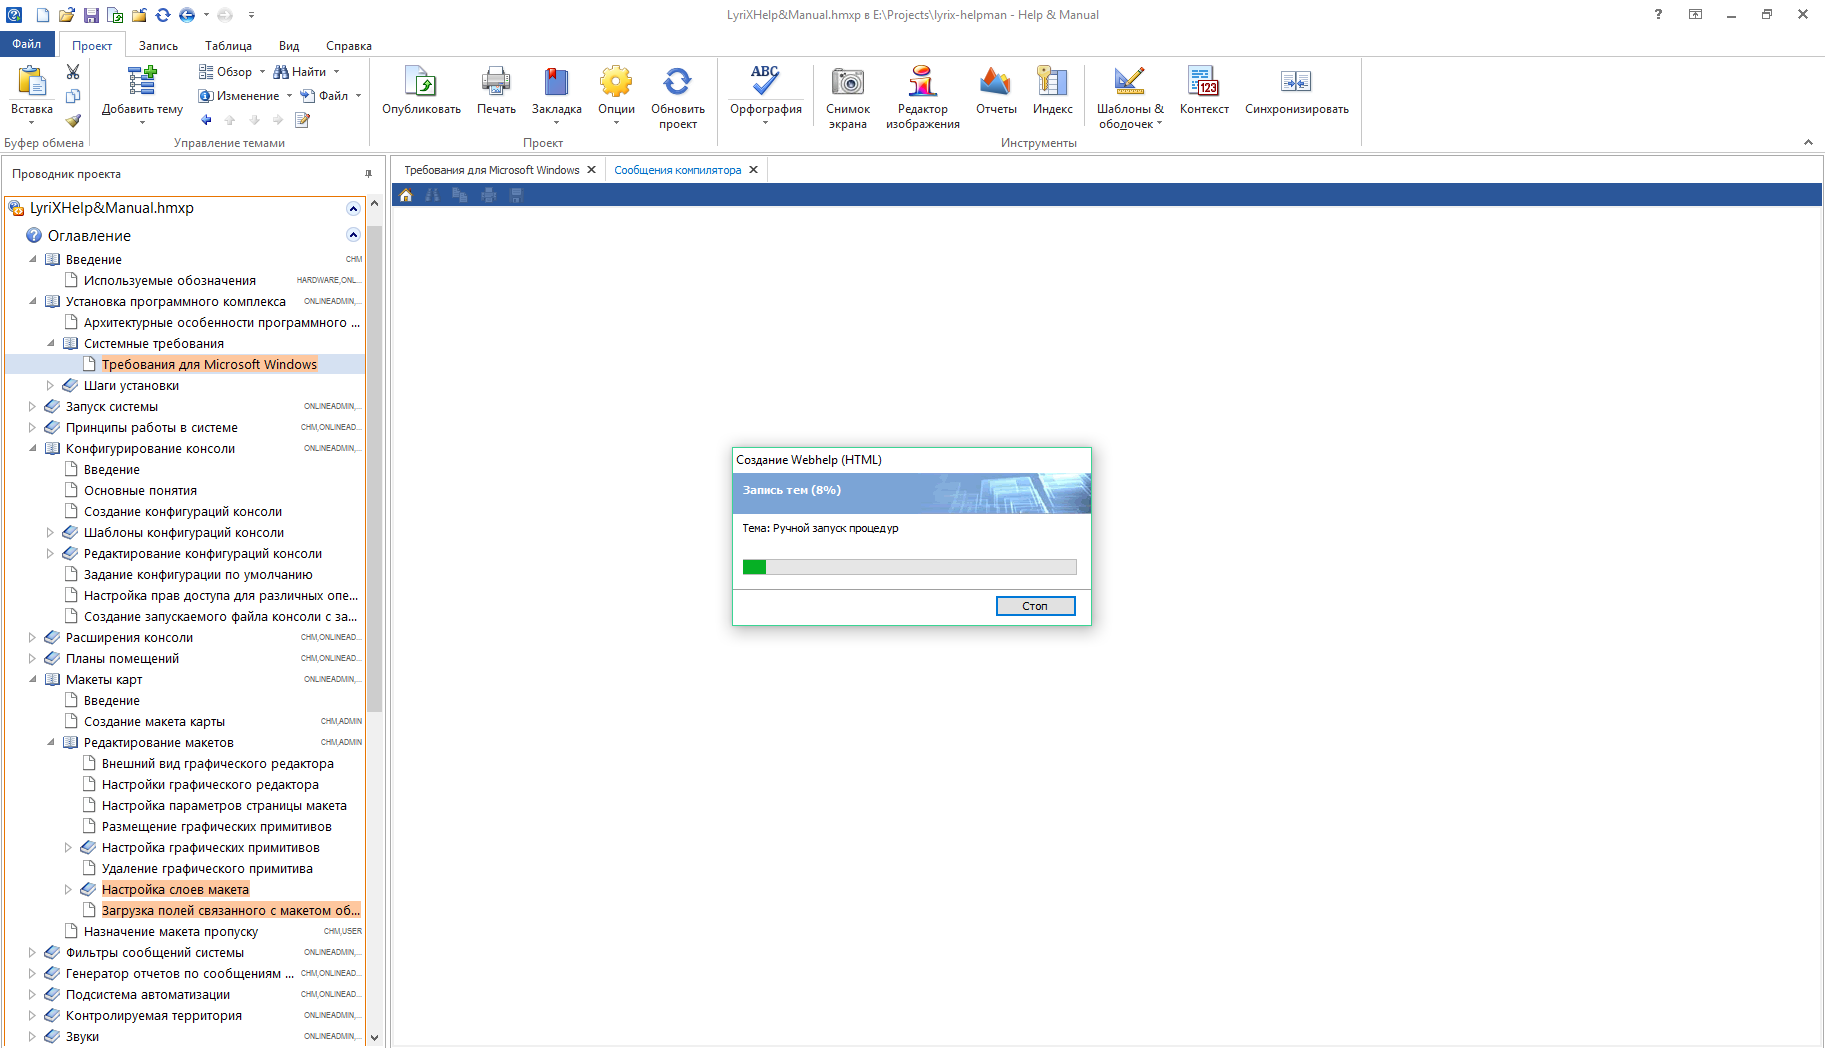
\includegraphics[width=0.7\linewidth]{images/creation}
			\caption{Структура проекта}
			\label{fig:creation}
		\end{figure*}
	
		\FloatBarrier
	
		Для каждого раздела может быть задан тег. С помощью разных комбинаций тегов можно управлять конфигурацией сборки. Это полезно тогда, когда есть несколько версий документа. Например, урезанное руководство для стандартных пользователей и расширенное для администратора.
				
		\begin{figure*}[h]
			\centering
			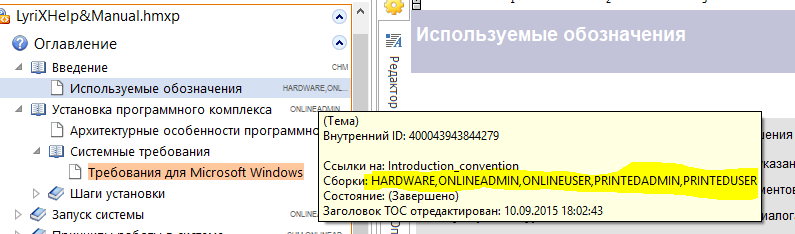
\includegraphics[width=0.7\linewidth]{images/multiple-builds}
			\caption{Множество конфигураций сборки}
			\label{fig:multiple-builds}
		\end{figure*}
	
	
		\FloatBarrier
		Один из вариантов публикации - формат WebHelp. Гипертекст в формате WinHelp реализуется в виде файла с расширением HLP (help-файла). HLP-файл формируется на основе файлов с текстом в формате RTF с помощью специального компилятора.
	
		\begin{figure*}[h]
			\centering
			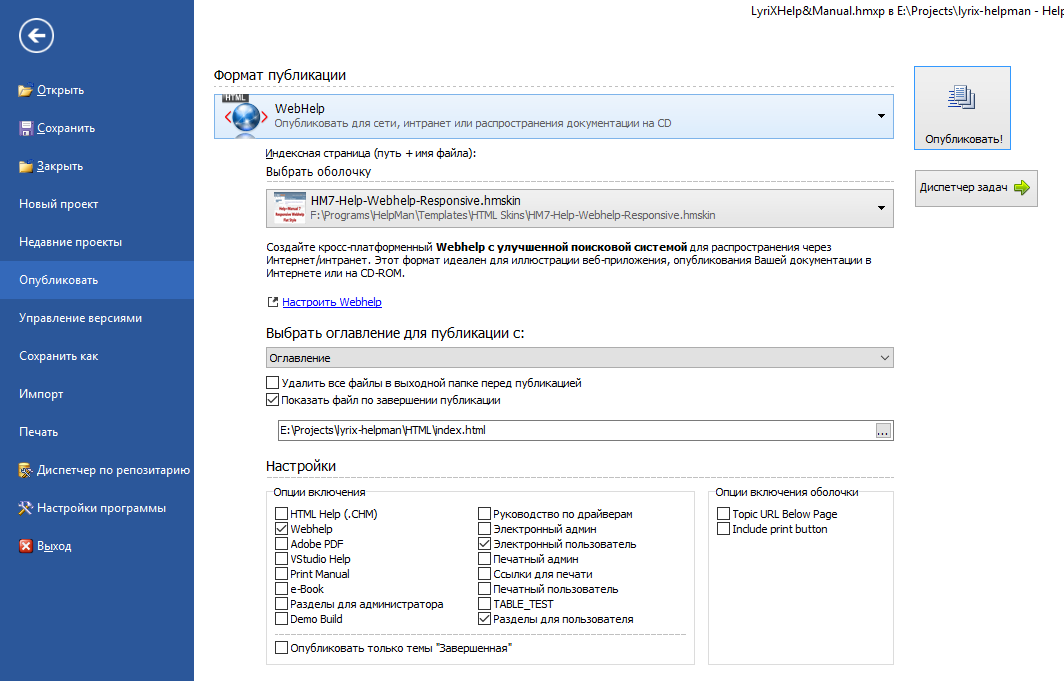
\includegraphics[width=0.7\linewidth]{images/publishing}
			\caption{Публикация в формате WebHelp}
			\label{fig:publishing}
		\end{figure*}
	
		\FloatBarrier
	
		Ниже приведены элементы навигации для такого документа.
	
		\begin{figure*}[h]
			\centering
			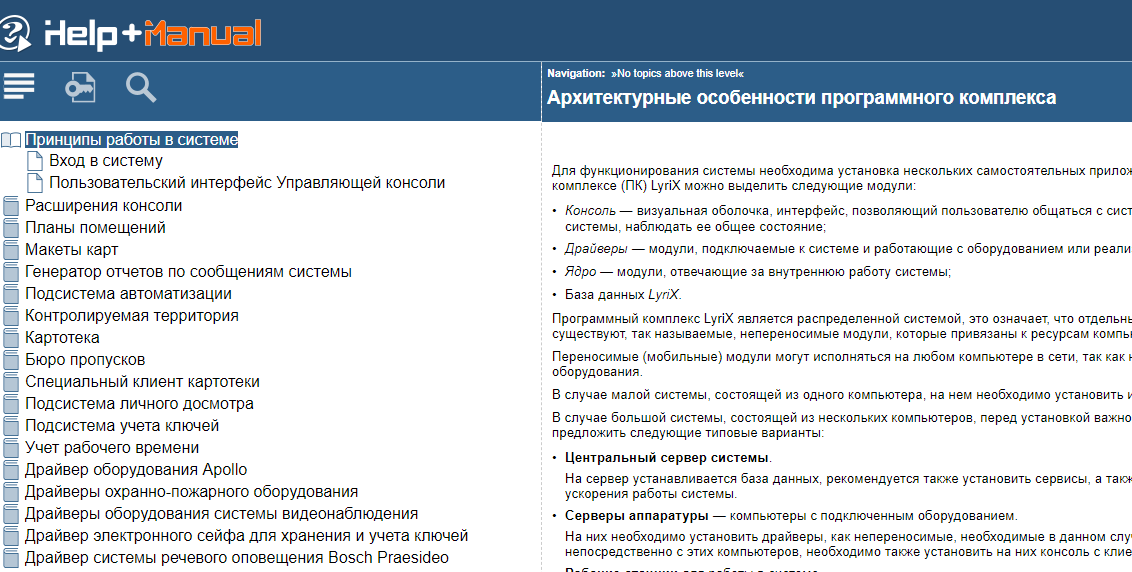
\includegraphics[width=0.7\linewidth]{images/table-of-content}
			\caption{Содержание}
			\label{fig:table-of-content}
		\end{figure*}
		\begin{figure*}[h]
			\centering
			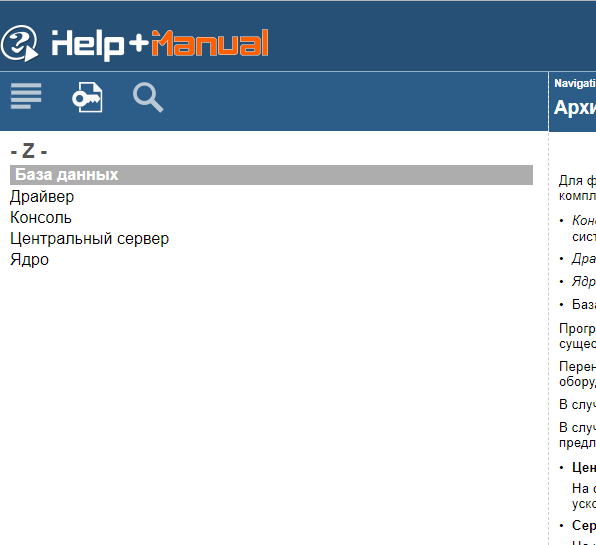
\includegraphics[width=0.7\linewidth]{images/ketword-index}
			\caption{Тезариус}
			\label{fig:ketword-index}
		\end{figure*}
		\begin{figure*}[h]
			\centering
			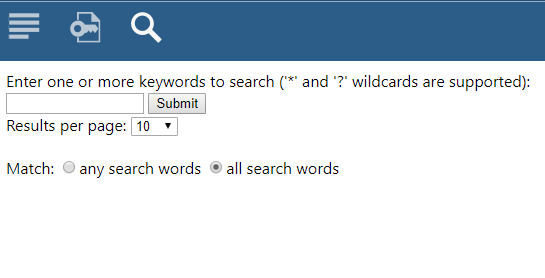
\includegraphics[width=0.7\linewidth]{images/search}
			\caption{Поиск}
			\label{fig:search}
		\end{figure*}
	
		\FloatBarrier
		
		\lstinputlisting[language={XML},caption={Пример страницы <<Введение>>},label={list:example}]{listings/example.xml}
		
	\section{Вывод}
	\begin{itemize}
		\item Гипертекстовая разметка (в частности справочник) очень удобна при разработке мануалов по использованию программных комплексов.
		\item Help \& Manual имеет полный набор средств по разработке справочника и не нуждается в дополнительных программных комплексах. Также он позволяет гибко формировать выходные документы и связывать справочную информацию.
	\end{itemize}
	